\documentclass[pdf,blends]{prosper}
\DefaultTransition{Box}
\usepackage[czech]{babel}
\usepackage[utf8]{inputenc}
\usepackage{color}
\usepackage{graphics}
\usepackage{picture}
\usepackage{amsfonts}
\usepackage{wasysym}
\title{Vlastnosti energy drinků}
\subtitle{Typografie a publikování \,--\, 5. projekt}
\author{Petr Knetl}
\date{28. dubna 2017}

\begin{document}
\maketitle
\begin{slide}{Co to je energy drink?}
\begin{itemize}
\item nealkoholický nápoj
\item vysoký obsah cukru (až patnáct kostek cukru na 500~ml)
\item kofein, taurin, guarana, yerba maté
\end{itemize}    
\begin{figure}[ht]
\begin{center}
\scalebox{1.3}{
\includegraphics{drink.eps}}
\end{center}
\end{figure}
\end{slide}

\begin{slide}{Povzbudivé účinky}
\begin{itemize}
\item zvýšení obsahu cukru v krvi $\rightarrow$ nabuzení organismu
\item krátkodobé zvýšení výkonu
\item uvolnění adrenalinu
\item zrychlení proudění krve
\item zvýšený přísun kyslíku mozku a svalům
\end{itemize}    

\end{slide}

\begin{slide}{Proč nepít energy drinky:}
\begin{itemize}
\item po vyprchání účinku přichází vyšší únava než před pozřením
\item vysoké množství kofeinu silně zatěžuje kardiovaskulární systém
\item způsobují nespavost
\item zvýšená nervozita a podrážděnost
\end{itemize}    
\begin{figure}[ht]
\begin{center}
\scalebox{0.4}{
\includegraphics{nope.eps}}
\end{center}
\end{figure}
\end{slide}

\begin{slide}{Kombinace s alkoholem:}

\begin{itemize}
\item snížení vnímavost opilosti
\item rychlejší vstřebávání alkoholu
\item pokračování konzumace alkoholu i přes vysokou opilost
\item projevy: zvýšená agresivita, poruchy srdečního rytmu, mdloby až ztráta vědomí

\end{itemize}

\end{slide}

\begin{slide}{Zvláště nevhodné~pro:}

\begin{itemize}
\item těhotné ženy
\item děti
\item lidi se slabý srdcem
\item diabetiky

\end{itemize}

\begin{figure}[h]
\center{\scalebox{0.19}{
\includegraphics{nochild.eps}} \quad \scalebox{0.3}{
\includegraphics{nopregnant.eps}}}
\end{figure}

\end{slide}


\begin{slide}{Děkuji za pozornost~\smiley}


\begin{figure}[h]
\center{\scalebox{0.4}{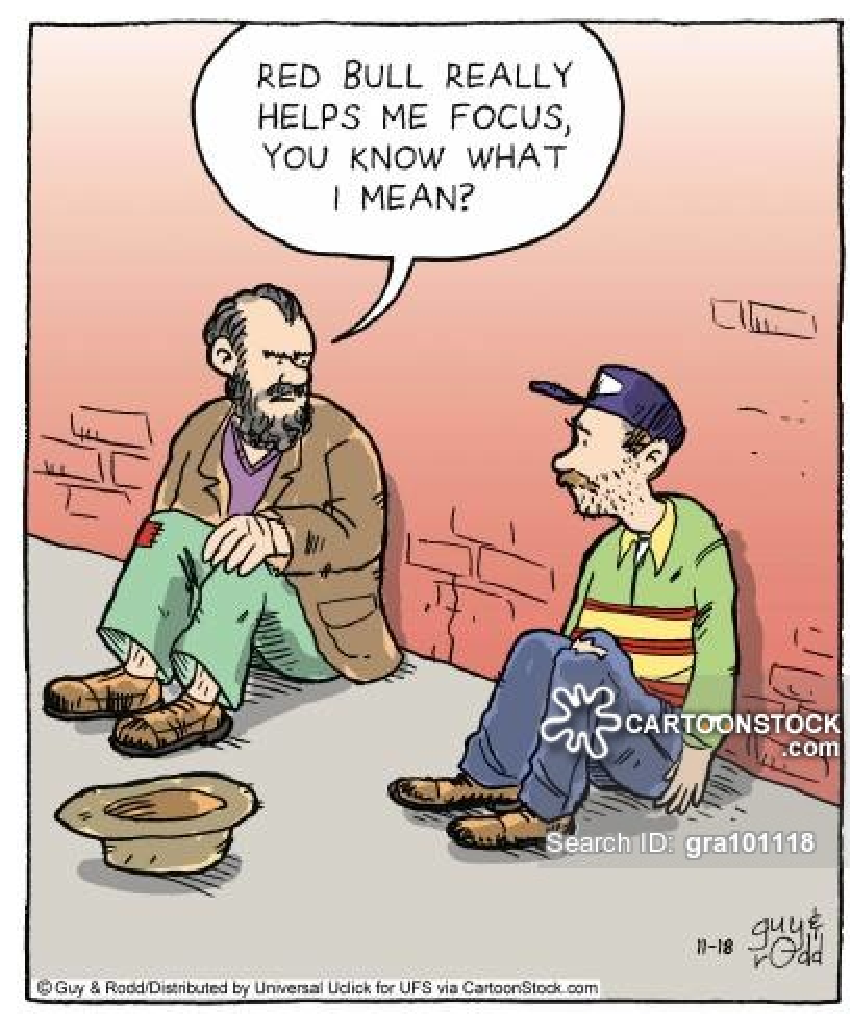
\includegraphics{energyhelp.eps}}}
\end{figure}

\end{slide}








\end{document}
